\section{Przypadek Testowy 2 - Algorytm genetyczny - zależność PRD od użytej metody selekcji}
  \subsection{Cel:}
    W tej części zostaną ze sobą porównane PRD rozwiązania algorytmu genetycznego w zależności użytej metody selekcji.
    \subsection{Założenia:}
    Do badania tego przypadku została wykorzystana instancja \textbf{berlin52.tsp}. Dodatkowo współczynnik selekcji został ustalony na 0.95. Ponad to wielkość populacji została ustalona na 10, liczba iteracji to 10000. Zmienne współczynniki mutacji \(m \in {0.05, 0.15, 0.25 ... 0.95}\) oraz 2 metody selekcji. Dla każdej wielkości współczynnika mutacji test został przeprowadzony trzykrotnie.
    \subsection{Metody selekcji:}
    \subsubsection{Ruletka:}
    Metoda selekcji przedstawicieli populacji polega na znormalizowaniu współczynnika dopasowania tak że suma wszystkich wynosi 1 odwrotnie proporcjonalnie do długości ścieżki. Następnie losowana jest liczba z przedziału \( [0, 1)\). Do nowej populacji dopisywana jest jedna ścieżka aż nowa populacja będzie tego samego rozmiaru co poprzednia.
    \subsubsection{Odcięcie:}
    Metoda selekcji przedstawicieli populacji polega na posortowaniu populacji względem długości rozwiązania i odcięcie sparametryzowanej najgorszej części (np. 10\%). aby uzupełnić populację najlepsze odobniki są doklejane po raz kolejny.
  \subsection{Wyniki: }
  Poniższa tabela przedstawia wyniki testów, odchylenie standardowe oraz błęd standardowy.
  \begin{table}[!ht]
    \centering
    \begin{tabular}{|l|l|l|l|l|l|l|}
    \hline
        m & R & SD\textsubscript{R} & SE\textsubscript{R} & O & SD\textsubscript{O} & SE\textsubscript{O} \\ \hline
        0.05 & 208.90 & 7.58 & 4.38 & 48.47 & 1.54 & 0.89 \\ \hline
        0.15 & 207.63 & 6.68 & 3.86 & 39.30 & 16.07 & 9.28 \\ \hline
        0.25 & 205.91 & 2.91 & 1.68 & 36.01 & 18.63 & 10.76 \\ \hline
        0.35 & 196.12 & 8.89 & 5.13 & 41.24 & 19.61 & 11.32 \\ \hline
        0.45 & 197.33 & 4.13 & 2.38 & 38.39 & 3.52 & 2.03 \\ \hline
        0.55 & 190.82 & 17.28 & 9.98 & 52.92 & 24.27 & 14.01 \\ \hline
        0.65 & 196.19 & 6.80 & 3.92 & 60.43 & 8.97 & 5.18 \\ \hline
        0.75 & 191.50 & 4.34 & 2.50 & 68.26 & 13.21 & 7.62 \\ \hline
        0.85 & 197.37 & 11.00 & 6.35 & 70.17 & 4.90 & 2.83 \\ \hline
        0.95 & 197.44 & 11.80 & 6.81 & 86.56 & 6.82 & 3.94 \\ \hline
    \end{tabular}
    \caption{m - współczynnik mutacji, R - PRD dla selekcji przez ruletkę, SD\textsubscript{R} - odchylenie standardowe dla selekcji przez ruletkę, SE\textsubscript{R} - Błąd standardowy dla selekcji przez ruletkę, O - PRD dla selekcji przez odcięcie, SD\textsubscript{O} - odchylenie standardowe dla selekcji przez odcięcie, SE\textsubscript{O} - Błąd standardowy dla selekcji przez odcięcie}

  \end{table}
    Odchylenie standardowe oraz błąd standardowy zostały obliczone według wzorów: \\
    Odchylenie standardowe:
    \[ \sigma = \sqrt{\frac{\sum_{n = 1}^{3}(\bar{x} - x_n)^2}{3}} \]
    Błąd standardowe:
    \[ \sigma_{\bar{x}} = \frac{\sigma}{\sqrt{3}} \]

  \subsection{Wykresy: }
    \begin{figure}[H]
      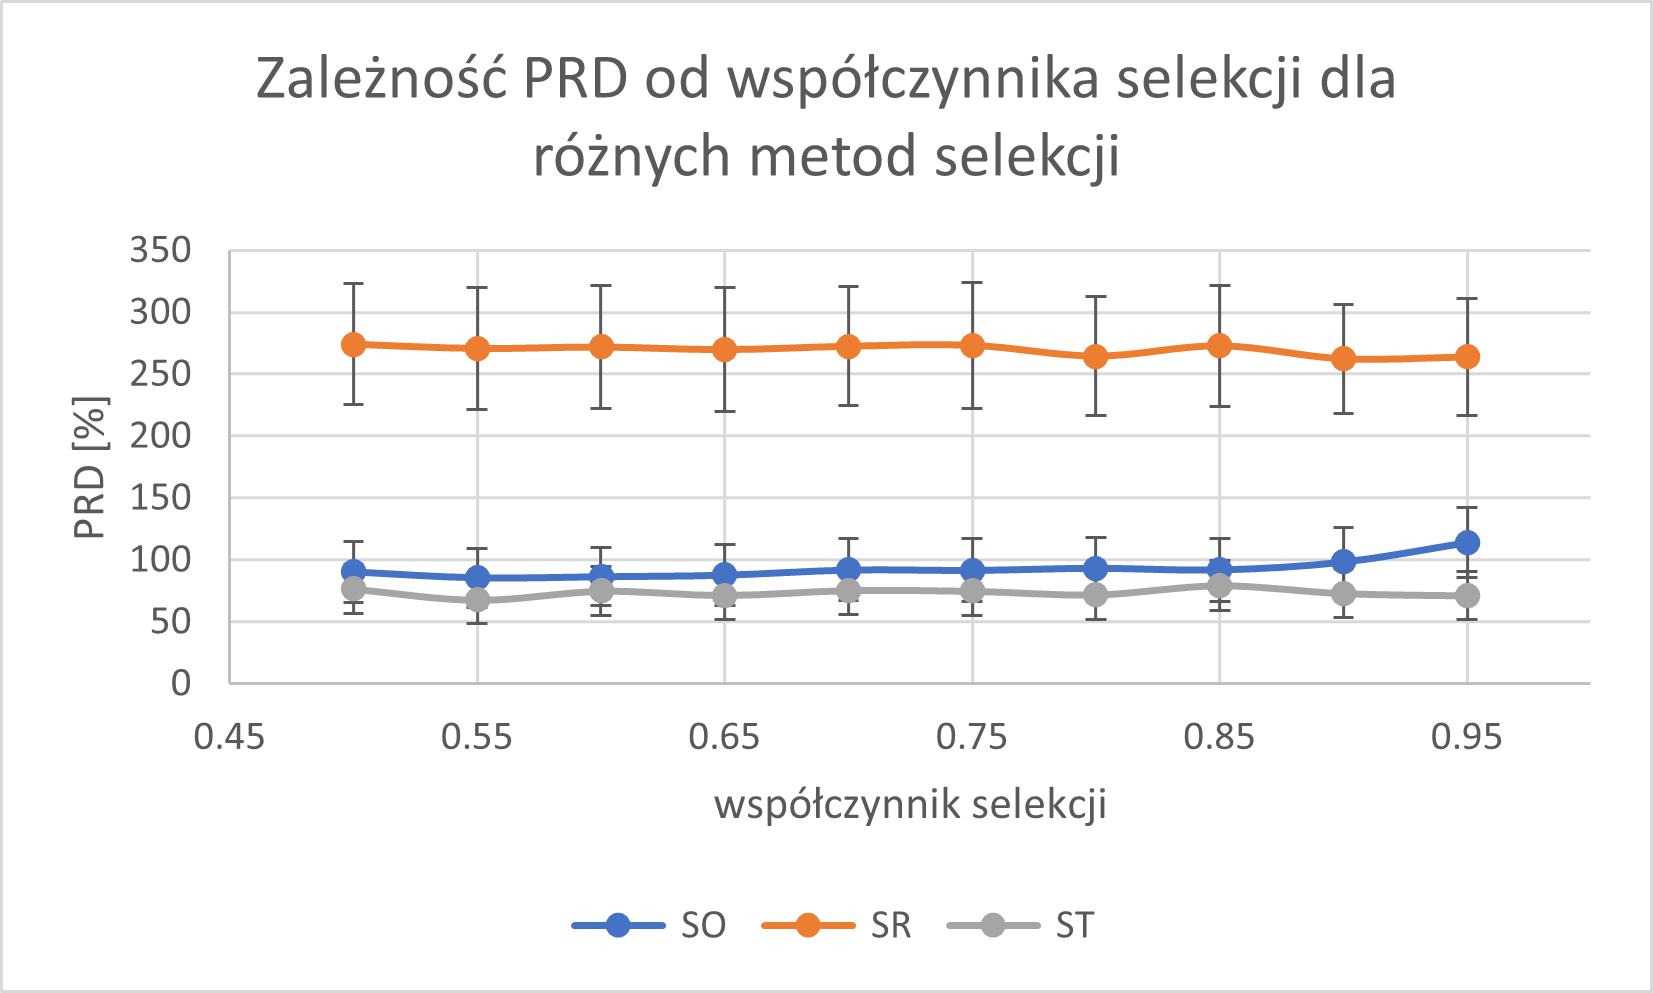
\includegraphics[scale=0.75]{chart_test_3.png}
      \centering
      \caption{zależność PRD od współczynnika mutacji}
    \end{figure}
  
    Na wykresach przedstawione są średnie wartości PRD dla badanych danych.
  \subsection{Wnioski: }
  Selekcja przez odcięcie sprawdza się zdecydowanie lepiej niż selekcja metodą ruletki. W metodzie ruletki najsłabsze osobniki mają szansę przejść do krzyżowania gdzie w metodzie odcięcia są zawsze usuwane i krzyżują się tylko najlepsze cechy.
